\section{Results analysis}\label{sec:resultAn}
\subsection{Model validation}
As the previous section shows, every graph simulated in Simulink presents the same shape as the presented in the original articles, so the model used in this article is valid. Note that there are small differences with the maximum and minimum values that the voltages have and some trajectories that do not fit with the compared graphs. These differences occur due to several reasons that do not diminish the validation of the model. It is considered important to explain the reasons this differences may take place.

In first place, chaotic systems are highly sensitive to small changes in the parameters and initial conditions. The problem is when the system is simulated for every iteration it needs information of every state prior; and, if the system simulated is chaotic every minor approximation that the software makes for a certain iteration influence the posterior iterations value more heavily than other systems. Therefore, the chaotic nature of the attractor makes it difficult to replicate exact graphs from other work.

In second place, other articles do not specify what algorithm they used to solve their equation and, as it is seen in section \ref{subsec:methods}, the algorithm used to solve the differential equation affects the solution (specially if the system is chaotic as the equations used in this paper). And even if the algorithm is specified in the article, like in \cite{rossler1976equation}, the author do not specify the step that he used in the algorithm that also changes the simulation as seen in SECTION EULERDIFERENTEPASO.

Therefore, the problems explained are not related to the implementation of the model worked instead problems inherent to simulation of chaotic systems. Consequently, the model is validated. 

%%%%%%%%%%%%%%%%%%%%%%%%%%%%%%%%%%%%%%%%%%%%%%%%%%%%%%%%%%%%%%%%%%%%%%%%

\subsection{Input Variation}
\subsubsection{Sines Inputs}
As it was presented in section \ref{subsubsec:sines}, both sine inputs make the system fall into a periodic orbit; this is due to the system no having enough time to create a chaotic behavior. It is constantly changing values from voltages that are known to cause chaotic behavior and some that do not. As the sine wave has an offset of $500V$, the average value is exactly $500V$; hence, as the input is much higher than the original $V_{cc0}$ and then the circuit charges and discharges quite often.

Between the two simulations performed (Figs. \ref{fig:3dSin2f} and \ref{fig:3dSin5f}), the sine input with less frequency ($2\text{rad}*s^{-1}$) could achieve a ``simpler'' orbit, since the system had a bit more time to attempt to follow an orbit alike the reference (Figs. \ref{fig:RosslerO} and \ref{fig:3DRosslerO}; unlike the input with higher frequency, where the system immediately falls into a more complex orbit.

\subsubsection{Step Input}\label{subsubsec:stepAn}
As it is shown in section \ref{subsubsec:step}, the step input provides an effective controller for the system in stationary state. It can be observed that the output signal Fig. \ref{fig:outStep} stabilizes shortly after the input is applied; and as well for the phase portrait \ref{fig:3dStep}, since it converges to a point in space. The stabilization is a result of the circuit charging immediately: the voltage is so high that it will not create dynamic behavior through the nodes; it is constant.


%%%%%%%%%%%%%%%%%%%%%%%%%%%%%%%%%%%%%%%%%%%%%%%%%%%%%%%%%%%%%%%%%%%%%%%%

\subsection{Parameter Variation}
It is important to highlight, that for the variation the parameters the values picked cannot be unusually big or small as resistance have a physical limitation for their values. In this manner, there is a threshold for what the minimum and maximum values can the resistances have without breaking the limitations of the system.

\subsubsection{Parameter \texorpdfstring{$R_a$}{Ra}}
It is seen that as the value for the resistance $a$ increases, the system changes for a more chaotic response to a periodic one as seen in figure \ref{fig:paraAvar}. This result does not come as a surprise, as it is consistent with the known circuits theory. As $R_a$ takes higher values, the current that moves around the circuit is lower due to the high resistance that the system has because of Ohm's Law. Therefore, the differences between the voltages in different times of the nodes are smaller, making the system periodic. Consequently, resistance $a$ acts as a controller as for increasing values of this state variable the system easily starts to change its chaotic nature.

This characteristic is more evident when the system is simulated with the same parameters but, increasing the time of simulation as in figure \ref{fig:ra500}. In this figure, the simulation is made with exactly the same parameters as in \ref{fig:3dparaAvard} but with the time of simulation 5 times the original. And, as it is seen, the graphic is totally identical to the original; then, this resistance makes the system completely oscillatory even for longer times therefore completely controlling it for increasing values.

\begin{figure}[H]
    \centering
    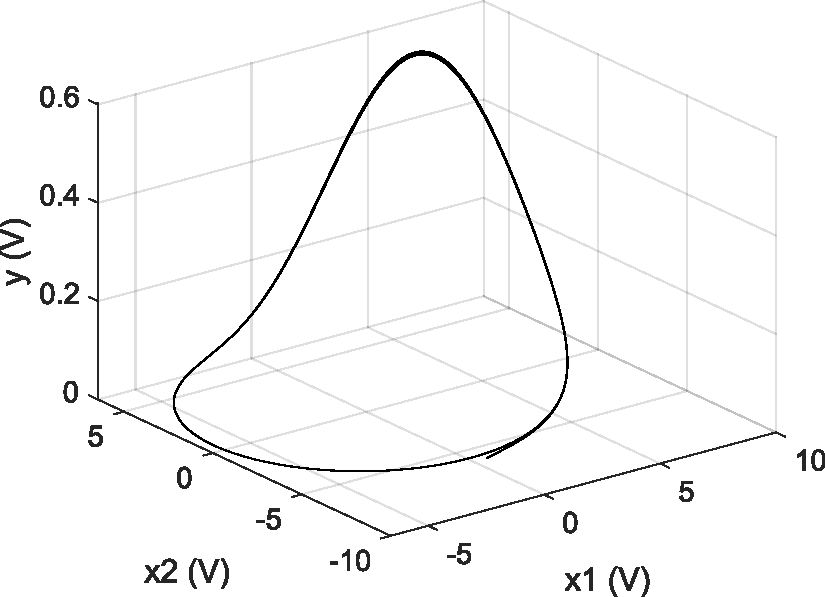
\includegraphics[scale=0.5]{figs/ra3652t500.pdf}
    \caption{3D results for $R_a4$ with final time 500.}
    \label{fig:ra500}
\end{figure}

\subsubsection{Parameter \texorpdfstring{$R_c$}{Rc}}
For decreasing values of $R_c$ it is seen that the values of the output increase. This is consistent with Ohm's law, as with lower resistance in the system the voltage is higher as there's more current in the circuit. In this manner, the first signal for $y$ takes more time to show; however, the output signal, as stated in \cite{canals2014random}, is difficult to predict therefore understanding the nature of why this occur is almost impossible.

On the other hand, when the value of this resistance is increased it occurs a phenomenon similar with $R_a$ but, instead of having an immediate periodic behaviour it has some high peaks at the start and then proceeds to control itself as in \ref{fig:paraCvarUpd}. As stated before, the output signal is difficult to predict therefore is not possible to attribute why this peaks happen. Still, it is consistent that the voltage of the output becomes periodic and with small peaks for the same reason that with $R_a$.

Taking this into account, this resistance is harder to predict how it affects the system at the start but, when time passes it takes the expected behaviour. This happens because these parameter affects the non-linear equation, therefore changes done to its value does not make linear changes. On the other hand, $R_a$ changes a linear equation making it quite easy to predict the changes that this value makes to the system.

%%%%%%%%%%%%%%%%%%%%%%%%%%%%%%%%%%%%%%%%%%%%%%%%%%%%%%%%%%%%%%%%%%%%%%%%

\subsection{Limit for Parameter Variation}

\subsubsection{Parameter \texorpdfstring{$R_a$}{Ra}}
As it is seen in \ref{fig:outParaAdown} the output $y$ have a increasing value, tending to infinity. This makes sense, as the resistance $a$ is really low, therefore the same argument is applied as the one in the parameter variation. A analogous argument can be applied for the upper bound. 

The problem with this found interval, is that it is known that this interval presents a range of values for which the system converges but, it is not sure that every value inside this range has a chaotic behavior. To found this interval it would be needed to make a partition of this interval with graphs with similar behaviour and, observe how chaotic is it (calculating the Lyapunov's Exponent) and categorizing it. But, the interval $[259.098131084k\Omega,10000k\Omega]$ is a superset for the set of the values of $R_a$ that makes the system keep its chaotic behaviour.

\subsubsection{Parameter \texorpdfstring{$R_b$}{Rc}}
With this parameter, it can be argued similarly as the one before.

%%%%%%%%%%%%%%%%%%%%%%%%%%%%%%%%%%%%%%%%%%%%%%%%%%%%%%%%%%%%%%%%%%%%%%%%
\subsection{Euler's and Runge-Kutta's Methods}
Section \ref{subsec:methods} shows the simulation results for both methods in both scenarios; Fig. \ref{fig:MethodMethod}. a) shows that, for the Euler method, the numerical solutions for the state equation are equivalent: both scenarios showed identical results since the output signals overlap.

For the Runge-Kutta's method, the results obtained are quite different. As Fig. \ref{fig:MethodMethod} b) shows, both methods match on the peaks localization, but differ on their magnitude. Roughly, for $30s<t<70s$, the difference can be easily perceived.

As it has been already explained, the main feature of chaotic systems is their sensitivity to small changes; the Runge-Kutta's algorithm has to do significantly more calculations, which implies that the propagation of error is much more notorious. As Simulink's implementation of this method is not known, it is tough to determine exactly what causes the difference with further implications; moreover, Simulink's method must have better handling of data and operations, since it must take advantage of the software features, and the algorithm implemented lacks efficiency.

